En esta etapa, se lleva a cabo la implementación del diseño del proceso ETL previamente definido, utilizando las herramientas seleccionadas. Se desarrollan los flujos de extracción, transformación y carga de los datos según lo establecido en el diseño.

Una vez implementado, se procede a realizar pruebas exhaustivas para garantizar el correcto funcionamiento del proceso. Estas pruebas incluyen la verificación de la extracción de datos de las fuentes, la correcta aplicación de las transformaciones definidas y la carga exitosa de los datos en el destino final.

El objetivo de las pruebas es asegurar que el proceso ETL cumpla con los requisitos establecidos y que los resultados obtenidos sean los esperados. Esto implica validar la integridad y coherencia de los datos transformados, así como verificar el rendimiento y la escalabilidad del proceso.

En caso de encontrar inconvenientes o desviaciones durante las pruebas, se realizan los ajustes necesarios en el diseño o en la configuración de las herramientas utilizadas. Es fundamental realizar iteraciones y pruebas adicionales hasta obtener resultados consistentes y satisfactorios.

Como primer paso en la construcción del proceso ETL, se importan las bibliotecas pandas y numpy para trabajar con el dataset. Luego se le da nombre a las columnas, ya que el contenido del archivo csv solo trae los datos. Una vez nombradas las columnas se ordenan para un entendimiento más facil del conjunto de datos, quedando de la siguiente manera respectivamente: rut, fecha, metodo, canal.

Ahora se comprueba la existencia de valores nulos en el dataframe, resultando lo siguiente:

\begin{figure}[H]
    \begin{minipage}[t]{0.8\textwidth}
        \caption{Valores nulos en el conjunto de datos.}
        \label{valoresNulos}        
    \end{minipage}

    \vspace{10pt}

    \centering
    \begin{minipage}[b]{0.4\textwidth}
        \centering
        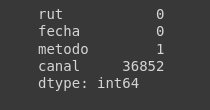
\includegraphics[width=\textwidth]{img/valores-nulos.png}        
    \end{minipage}

    \begin{minipage}[t]{0.9\textwidth}
        Fuente: Elaboración propia.
    \end{minipage}
\end{figure}

Como se puede ver en la imagen anterior solamente los campos 'metodo' y 'canal' poseen valores nulos, de hecho, el primero solo cuenta con un valor nulo. La columna 'canal' cuenta con 36,852 valores nulos. Luego de eliminar los valores nulos se pasa a eliminar las filas que contengan métodos inconsistentes o irrelevantes, que son:
\begin{itemize}
    \item reCaptcha()
    \item clientes/surveys
    \item clientes/cuentas/validar-cuenta-corriente
    \item clientes/cuentas/cuentas-bancarias
    \item clientes/cuentas/cuentas-bancarias?rut=******** 
    \item clientes/cuentas/cuentas-bancarias?rut=********
    \item clientes/cuentas/cuentas-bancarias?rut=*********
    \item clientes/cuentas/cuentas-bancarias?rut=*********
    \item clientes/cuentas/cuentas-bancarias?rut=*********
    \item clientes/cuentas/cuentas-bancarias?rut=********
    \item clientes/cuentas/cuentas-bancarias?rut=*********
    \item clientes/cuentas/cuentas-bancarias?rut=*********
    \item clientes/cuentas/APV/solicitud/giros?rut=*********\&account=APV
    \item clientes/cuentas/cuentas-bancarias?rut=*********
\end{itemize}

Es importante mencionar que el método reCaptcha() de Google valida la autenticidad de usuarios frente a bots, pero su utilidad se limita a la seguridad en línea. No ofrece información relevante para predecir el comportamiento de los usuarios en la plataforma, siendo necesario recurrir a los otros datos para comprender mejor sus acciones y patrones de uso.

Ahora se continua con la estandarización del formato de la fecha, quedando con el formato UTC (YYYY-MM-DDTHH:MM:SS.sssZ). La estandarización del formato de la fecha es un paso esencial para garantizar la coherencia y la compatibilidad de los datos. En este caso, se ha optado por este formato debido a una convención global reconocida que asegura la uniformidad y comprensión en diferentes contextos y aplicaciones.

Después de ajustar el formato de la fecha, se procede a corregir la denominación incorrecta de ciertos métodos registrados. Estos métodos son: WEB-Actualizacion-datos y WEB-Contacto-tramite-pensión. Ambos valores registrados en el campo 'canal' presentaron errores de registro. Este problema fue identificado tras el análisis del conjunto de datos, y se informó a la empresa para que corrigiera este error. En la plataforma, únicamente existen dos canales de acceso: 'WEB' y 'PWA'. El primero corresponde a la página web de la plataforma, mientras que el segundo se refiere a la aplicación. En consecuencia, se procede a modificar el nombre de los canales incorrectamente registrados (pertenecientes al canal 'WEB', según su nombre y confirmado con la empresa), para que se ajusten al nombre correcto de canal 'WEB'.

Al finalizar el proceso de ETL se puede ver la diferencia entre el dataset inicial y el dataset final. Primero se presenta una descripción incial del conjunto de datos, esto antes de construir y ejecutar el proceso ETL.

\begin{figure}[H]
    \begin{minipage}[t]{0.8\textwidth}
        \caption{Descripción del dataset antes del proceso ETL.}
        \label{describeInicial}        
    \end{minipage}

    \vspace{10pt}

    \centering
    \begin{minipage}[b]{0.8\textwidth}
        \centering
        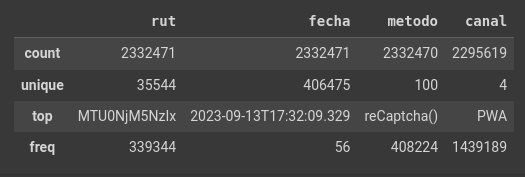
\includegraphics[width=\textwidth]{img/describe_data_inicial.png}        
    \end{minipage}

    \begin{minipage}[t]{0.9\textwidth}
        Fuente: Elaboración propia.
    \end{minipage}
\end{figure}

Ahora se presenta una descripción del conjunto luego del proceso ETL.

\begin{figure}[H]
    \begin{minipage}[t]{0.8\textwidth}
        \caption{Descripción del dataset después del proceso ETL.}
        \label{describeFinal}        
    \end{minipage}

    \vspace{10pt}

    \centering
    \begin{minipage}[b]{0.9\textwidth}
        \centering
        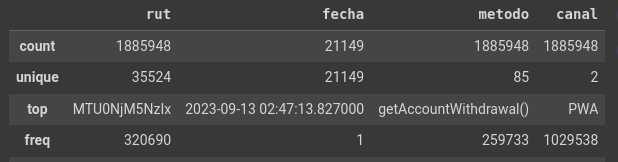
\includegraphics[width=\textwidth]{img/describe_data_final.png}        
    \end{minipage}

    \begin{minipage}[t]{0.9\textwidth}
        Fuente: Elaboración propia.
    \end{minipage}
\end{figure}

Después de aplicar el proceso ETL a los datos iniciales, se observan cambios notables en varias dimensiones del conjunto de datos. En primer lugar, el tamaño del conjunto de datos se redujo significativamente de 2,332,471 registros a 1,885,948, lo que sugiere una eficaz limpieza y eliminación de datos redundantes o inconsistentes. A nivel de valores únicos, la columna 'rut' mantuvo su estabilidad con 35,544 valores únicos, mientras que 'fecha' se estandarizó de 406,475 a 21,149 valores únicos, indicando una consolidación y uniformidad en el registro de fechas. Además, las columnas 'método' y 'canal' experimentaron reducciones significativas en la cantidad de valores únicos, pasando de 100 a 85 y de 4 a 2 respectivamente, lo que indica una simplificación y  una corrección de errores en la categorización. Los valores más frecuentes ('top') variaron en todas las columnas, destacando cambios notables en 'fecha', 'método' y 'canal', lo que indica una reestructuración significativa de los datos y posiblemente una mejora en la precisión y relevancia de la información.

Una vez completadas las etapas de limpieza y transformación mencionadas previamente, estamos listos para adentrarnos en el análisis de los datos. Este análisis es fundamental para extraer la información necesaria que orientará el desarrollo de un modelo de aprendizaje automático.